%
%TODO: work out diffraction circular aperture
%
%TODO: workout poisson noise
%
%TODO: workout conjugate gradients
%
%TODO: workout ransac
%
%TODO: workout belief propagation
%
%TODO: workout delauney
%
%TODO: workout splines
%

\section{Appendix}\label{sec:appendix}
\localtableofcontents

% \subsubsection{Rayleigh Criterion}

% \newcommand*{\E}{\bm{E}}
% \newcommand*{\B}{\bm{B}}
% \newcommand*{\rr}{\bm{r}}
% \newcommand*{\Ef}{\textit{\textbf{E}} }

% Starting with Maxwell's equations in a vacuum (in differential form) for the electric field \(\E(x,y,z, t)\) and the magnetic field \(\B(x,y,z, t)\):
% %
% \begin{align}
%     \nabla \times \B = \frac{1}{c^2} \frac{\partial \E}{\partial t} \\
%     \nabla \times \E = - \frac{\partial \B}{\partial t}
% \end{align}
% %
% Note that
% %
% \begin{equation}
%     \nabla \times \left( \nabla \times \E \right) = \pd{}{t} \left( \nabla \times \B\right) = \frac{1}{c^2} \pdv[2]{\E}{t}
% \end{equation}
% %
% and with the identity \(\nabla \times \nabla \times \E = \nabla (\nabla\cdot \E) - \nabla^2 \E\) we have the vector E-field \newterm{vector wave equation}:
% %
% \begin{equation}
%     \nabla^2 \E = \frac{1}{c^2} \pdv[2]{\E}{t}
% \end{equation}
% %
% This decouples each components of the \newterm{\textbf{E}} field. We therefore arbitrarily choose the \(z\) component and solve the \newterm{scalar wave equation} for \(E \coloneqq E_z\)
% %
% \begin{equation}
%     \nabla^2 E = \frac{1}{c^2} \pdv[2]{E}{t}\label{eqn:scalarwaveeqn}
% \end{equation}

% We seek \newterm{monochromatic wave solutions} of eqn ~\eqref{eqn:scalarwaveeqn}, i.e., those that are of such a form
% %
% \begin{equation}
%     E(\rr, t) = \psi(\rr) e^{-i \omega t}\label{eqn:monochromsol}
% \end{equation}
% %
% that the oscillatory component, \(e^{i \omega t}\) is only a function of \(\omega \coloneqq 2 \pi c / \lambda\) (\(\lambda\) is \newterm{wavelength} of the solution) and the \newterm{wave field} \(\psi(\rr)\) is only a function of \(\rr \coloneqq (x, y, z)\) spatial coordinates.
% %
% If \newterm{E} obeys eqn~\eqref{eqn:scalarwaveeqn} then \(\psi\) obeys the \newterm{Helmholtz equation}:
% %
% \begin{equation}
%     (\nabla^2 + k^2) \psi(\rr) = 0\label{eqn:helmholtz}
% \end{equation}
% %
% where \(k \coloneqq \omega / c\) is the \newterm{wavenumber} .
% %
% To solve the Helmholtz equation for \(\psi\) we use the method of \newterm{Green's functions}; we look for a solution \(G(\rr, \rr')\)
% %
% \begin{equation}
%     \nabla^2 G(\rr, \rr') + k^2 G(\rr, \rr') = -4 \pi \delta(\rr -\rr')\label{eqn:greenshelm}
% \end{equation}
% %
% where \(\delta\) is the Dirac delta \newterm{generalized function}\anote{diracdelta}.
% %
% Equation~\eqref{eqn:greenshelm} corresponds to a single point source at the position \(\rr' \coloneqq (x', y', z')\).
% %
% If we assume that \(G\) is only a function of displacement \(\bm{\rho} \coloneqq \rr - \rr'\) then we can introduce the Fourier integral representation \(\mathcal{G}\) of \(G\):
% %
% \begin{equation}
%     G(\rr) = \int\limits \mathcal{G}(\bm{\kappa})e^{i \bm{\kappa}\cdot \rho} \dif^{3}\kappa
% \end{equation}
% %
% Then using the fact that \(\mathcal{F} \left\{ \delta(\bm{\rho}) \right\} = 1\) we have
% %
% \begin{equation}
%     \mathcal{G}(\bm{\kappa}) = \frac{1}{2 \pi^2 } \frac{1}{\abs{\bm{\kappa}}^2 - k^2}
% \end{equation}

\subsection{Automatic Differentiation}\label{subsubsec:autodiff}

Let
%
\begin{align*}
    F\colon\; \bx \in \mathbb{R}^n \mapsto y \in \mathbb{R}
\end{align*}
%
and decompose \(F\) as
\begin{equation*}
    F = D \circ C \circ B \circ A
\end{equation*}
%
where
%
\begin{align*}
    A & \colon\; \bx \in \mathbb{R}^n \mapsto  \bm{a} \in \mathbb{R}^m    \\
    B & \colon\; \bm{a} \in \mathbb{R}^m \mapsto  \bm{b} \in \mathbb{R}^k \\
    C & \colon\; \bm{b} \in \mathbb{R}^k \mapsto  \bm{c} \in \mathbb{R}^j \\
    D & \colon\; \bm{c} \in \mathbb{R}^j \mapsto  y \in \mathbb{R}
\end{align*}
%
Let \(y_0 = F(\bm{x}_0)\) where \(\bx_0 \coloneqq \left( x_{01}, \dots, x_{0n}\right)\).
%
Then the gradient of \(F\) evaluated at \(\bx_0\) is
\begin{equation*}
    F'(\bm{x}_0) = \evalat[\bigg]{\pdv{y}{\bm{x}}}{\bx = \bx_0}
    = \left(
    \evalat[\bigg]{\pdv{y}{x_1}}{x_1 = x_{01}},
    \;\dots\dots\;,
    \evalat[\bigg]{\pdv{y}{x_n}}{x_n = x_{0n}}
    \right)
\end{equation*}
%
Note we are implicitly defining the parameter of \(F' = \pdv{y}{\bx}\) to be \(\bx\).
%
This is fine because parameters can be renamed at will\anote{boundvariable} but it's important to keep in mind that \(F'\) is wholly different from \(F\) and could have any other parameter.
%
By the chain rule
\begin{equation*}
    F'(\bm{x}_0) =  D'(C'(B'(A'(\bx_0))))
\end{equation*}
%
or if we define intermediate values
%
\begin{align*}
    \bm{a}_0 & = A(\bx_0)    \\
    \bm{b}_0 & = B(\bm{a}_0) \\
    \bm{c}_0 & = C(\bm{b}_0) \\
    y_0      & = D(\bm{c}_0)
\end{align*}
%
then
%
\begin{equation}
    F'(\bm{x}_0) =  \evalat[\bigg]{\pdv{y}{\bm{c}}}{\bm{c}=\bm{c}_0} \times\;
    \evalat[\bigg]{\pdv{\bm{c}}{\bm{b}}}{\bm{b}=\bm{b}_0} \times\;
    \evalat[\bigg]{\pdv{\bm{b}}{\bm{a}}}{\bm{a}=\bm{a}_0} \times\;
    \evalat[\bigg]{\pdv{\bm{a}}{\bm{x}}}{\bx=\bx_0} \label{eqn:chainruleproduct}
\end{equation}
%
where now a term like \(\evalat[\big]{\pdv{\bm{b}}{\bm{a}}}{\bm{a}=\bm{a}_0}\) is the \newterm{Jacobian} of \(B\) evaluated at \(\bm{a}_0\):
%
\begin{align*}
    \evalat[\bigg]{\pdv{\bm{b}}{\bm{a}}}{\bm{a}=\bm{a}_0}
     & = \evalat*{
        \begin{bmatrix}
            \pdv{b_1}{a_1} & \cdots & \pdv{b_1}{a_m} \\
            \vdots         & \ddots & \vdots         \\
            \pdv{b_k}{a_1} & \cdots & \pdv{b_k}{a_m}
        \end{bmatrix}
    }{\bm{a}=\bm{a}_0} \\
     & \coloneqq
    \begin{bmatrix}
        \evalat[\Big]{\pdv{b_1}{a_1}}{a_1 = a_{01}} & \cdots & \evalat[\Big]{\pdv{b_1}{a_m}}{a_m = a_{0m}} \\
        \\
        \vdots                                      & \ddots & \vdots                                      \\
        \\
        \evalat[\Big]{\pdv{b_k}{a_1}}{a_1 = a_{01}} & \cdots & \evalat[\Big]{\pdv{b_k}{a_m}}{a_m = a_{0m}} \\
    \end{bmatrix}
\end{align*}
%

The right hand side (RHS) of eqn.~\eqref{eqn:chainruleproduct} is associative; if we want to compute \(F'\) in general we can accumulate products starting from the right or starting from the left:
%
\begin{align}
    F' & = \pdv{y}{\bm{c}}
    \left( \pdv{\bm{c}}{\bm{b}}
    \left( \pdv{\bm{b}}{\bm{a}}
    \pdv{\bm{a}}{\bm{x}}\right)\right) \label{eqn:forwardaccum} \\
    F' & =  \left( \left( \pdv{y}{\bm{c}}
    \pdv{\bm{c}}{\bm{b}} \right)
    \pdv{\bm{b}}{\bm{a}} \right)
    \pdv{\bm{a}}{\bm{x}} \label{eqn:reverseaccum}
\end{align}
%
Computing \(F'\) as in eqn.~\eqref{eqn:forwardaccum} is called \newterm{forward accumulation} (because it parallels the evaluation order of \(F\)) and, conversely, deriving \(F'\) as in eqn.~\eqref{eqn:reverseaccum} is called \newterm{reverse accumulation}.
%
Notice that since \(F\colon\; \mathbb{R}^n  \rightarrow \mathbb{R}\) it's the case that while \(\pdv{\bm{b}}{\bm{a}}\cdot \pdv{\bm{a}}{\bm{x}}\) is a jacobian--jacobian product
\begin{equation}
    \pdv{\bm{b}}{\bm{a}}\cdot
    \pdv{\bm{a}}{\bm{x}} =         \begin{bmatrix}
        \pdv{b_1}{a_1} & \cdots & \pdv{b_1}{a_m} \\
        \vdots         & \ddots & \vdots         \\
        \pdv{b_k}{a_1} & \cdots & \pdv{b_k}{a_m}
    \end{bmatrix}
    \cdot
    \begin{bmatrix}
        \pdv{a_1}{x_1} & \cdots & \pdv{a_1}{x_n} \\
        \vdots         & \ddots & \vdots         \\
        \pdv{a_m}{x_1} & \cdots & \pdv{a_m}{x_n}
    \end{bmatrix}
\end{equation}
%
while \(\pdv{y}{\bm{c}}\cdot \pdv{\bm{c}}{\bm{b}}\) is a vector--Jacobian product (called a VJP)
%
\begin{equation}
    \pdv{y}{\bm{c}}\cdot
    \pdv{\bm{c}}{\bm{b}} = \left( \pdv{y}{c_1}, \dots,  \pdv{y}{c_j} \right)
    \cdot
    \begin{bmatrix}
        \pdv{c_1}{b_1} & \cdots & \pdv{c_1}{b_k} \\
        \vdots         & \ddots & \vdots         \\
        \pdv{c_j}{b_1} & \cdots & \pdv{c_j}{b_k}
    \end{bmatrix}
\end{equation}
%
All intermediate products will also be VJPs (for reverse accumulation); in general reverse accumulation is more efficient when the dimension of the domain is greater than the dimension of the range.

\subsection{Splines}\label{subsubsec:splines}

A \newterm{spline} is a piecewise defined polynomial function. For example a simple \newterm{order} \(d+1\) spline \(s\) could be defined
%
\[
    s(x) \coloneqq \sum_{i=0}^d \mathbbm{1}_{[k_j, k_{j+1})}P_{ij} \cdot (x - k_j)^i
\]
%
where the \(n+1\) increasing \newterm{knots} \(k_0 < \cdots < k_n\) bracket \(n\) intervals over which the component polynomials are defined, and the \((d+1)\) polynomial coefficients \(P_{ij}\) define the spline (see figure~\ref{fig:cubicspline}) for \(x \in [k_j, k_{j+1})\) (\(\mathbbm{1}\) enforces this\anote{indicator}).
%
Splines need not be differentiable (nor even continuous) at the knots but can be specified with such continuity constraints (at the knots).
%
The number of degrees of freedom of a spline over \(n+1\) knots and of order \(d+1\) (i.e., the dimension of the vector space\anote{vectorspace} of such splines) is the number of polynomial coefficients minus the number of continuity conditions.
%
For example if the spline is constrained to be maximally continuous (i.e., continuous and differentiable \(d-1\) times\anote{splinecontconstr}) then the spline has \(d+1\) polynomial coefficients for every one of the \(n\) knot intervals and \(d\) continuity constraints at every one of the \(n-1\) interior knots (continuity constraints cannot be specified at the boundary knots), which implies
%
\[
    n(d+1) - (n-1)d = n+d
\]
%
degrees of freedom. The spline construction naturally extends to dimensions greater than 1.

A Basic-spline (B-spline) is a spline defined as a linear combination of a particular set of basis functions: the B-spline basis element \(B_{i, d+1}\) of order \(d+1\) (degree \(d\)) over knots \(k_i < \cdots < k_{i+d+1}\) is defined recursively according to the Cox-de Boor recursion formula \cite{de1971subroutine}:
%
\begin{align}
    B_{j,1} (x)   & \coloneqq \mathbbm{1}_{[k_j, k_{j+1})}                         \\
    B_{j,d+1} (x) & \coloneqq \frac{x-k_j}{k_{j+d} - k_j} B_{j,d} (x)              \\
                  & \quad+ \frac{k_{j+d+1} - x}{k_{j+d+1} - k_{i+1}} B_{j+1,d} (x)
\end{align}
%
Note that the coefficients
%
\[
    \frac{x-k_j}{k_{j+d} - k_j}
\]
%
and
%
\[
    \frac{k_{j+d+1} - x}{k_{j+d+1} - k_{i+1}}
\]
%
interpolate smoothly between the lower order B-splines \(B_{j,d}, B_{j+1,d}\) as \(x\) goes from \(k_j\) to \(k_{j+d+1}\).

\begin{figure}
    \centering
    \begin{adjustbox}{width=\linewidth}
        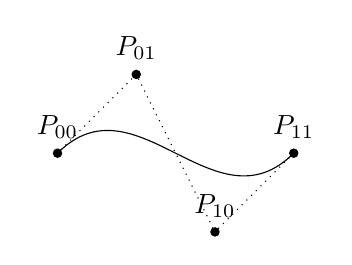
\begin{tikzpicture}
            \tikzset{
                ctrlpoint/.style={%
                        draw=black,
                        fill,
                        circle,
                        inner sep=0,
                        minimum width=3pt,
                    }
            }
            \newcommand\Bezier[4]{% \bezier (lowercase 'b') was already defined elsewhere
                \node (p1) [ctrlpoint,label=90:\(P_{00}\)] at (#1) {};
                \node (p2) [ctrlpoint,label=90:\(P_{01}\)] at (#2) {};
                \node (p3) [ctrlpoint,label=90:\(P_{10}\)] at (#3) {};
                \node (p4) [ctrlpoint,label=90:\(P_{11}\)] at (#4) {};
                \draw [black, dotted] (p1) -- (p2) -- (p3) -- (p4);
                \draw [black] (#1) .. controls (#2) and (#3) .. (#4);
            }
            \Bezier{0,0}{1,1}{2,-1}{3,0}
        \end{tikzpicture}
    \end{adjustbox}
    \caption{Cubic spline.}
    \label{fig:cubicspline}
\end{figure}

\subsection{Delaunay Triangulation}\label{subsec:delaunay}

Delaunay triangulation for a set points in the plane is a such that no point in is inside the circumcircle of any triangle in triangulation (see figure~\ref{fig:delaunaycircum}).
%
\begin{figure}[htbp]
    \centering
    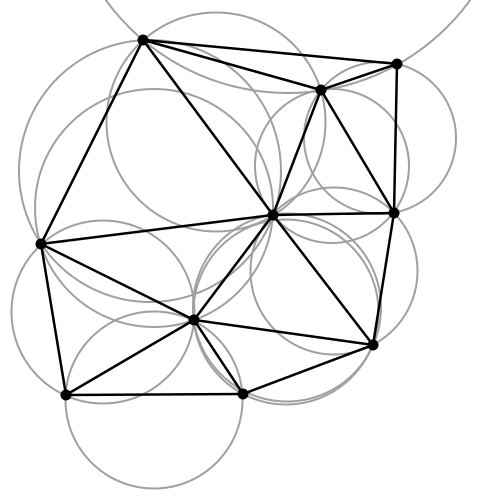
\includegraphics[width=\linewidth]{figures/appendix/delaunay.png}
    \caption{Delaunay Triangulation.}\label{fig:delaunaycircum}
\end{figure}
%
A local characterization two triangles ABD and BCD with the common edge BD (see figure~\ref{subfig:delauneymismatch}), if the sum of the angles \(\alpha\) and \(\gamma\) is less than or equal to \(\ang{180}\), the triangles meet the Delaunay condition.
%
\begin{figure}[htbp]
    \centering
    \newcommand*{\subfigwidth}{.8\linewidth}
    \begin{subfigure}[b]{\subfigwidth}
        \centering
        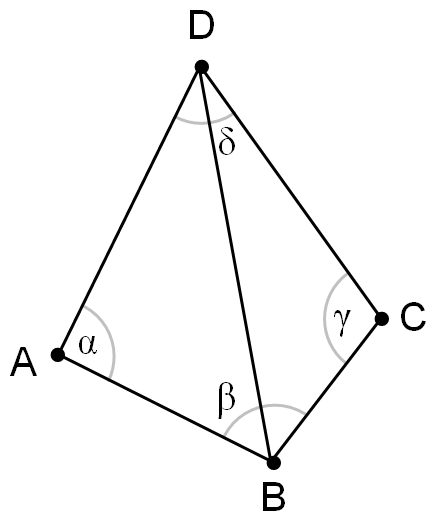
\includegraphics[width=\subfigwidth]{figures/appendix/Delaunay_geometry.png}
        \caption{This triangulation does not meet the Delaunay condition (the sum of \(\alpha\) and \(\gamma\) is bigger than \(\ang{180}\)).}\label{subfig:delauneymismatch}
    \end{subfigure}

    \begin{subfigure}[b]{\subfigwidth}
        \centering
        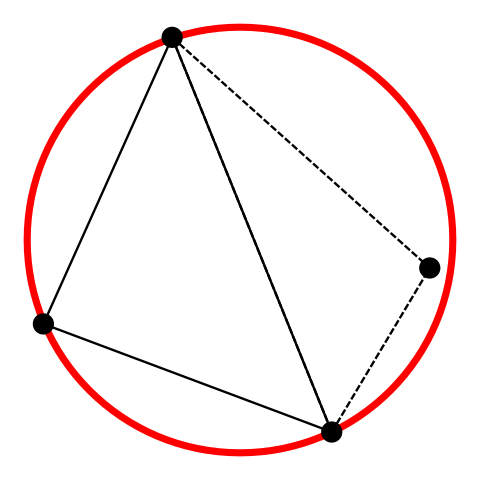
\includegraphics[width=\subfigwidth]{figures/appendix/Point_inside_circle_-_Delaunay_condition_broken.png}
        \caption{This pair of triangles does not meet the Delaunay condition (the circumcircle contains more than three points).}\label{subfig:delauneyflip}
    \end{subfigure}

    \begin{subfigure}[b]{\subfigwidth}
        \centering
        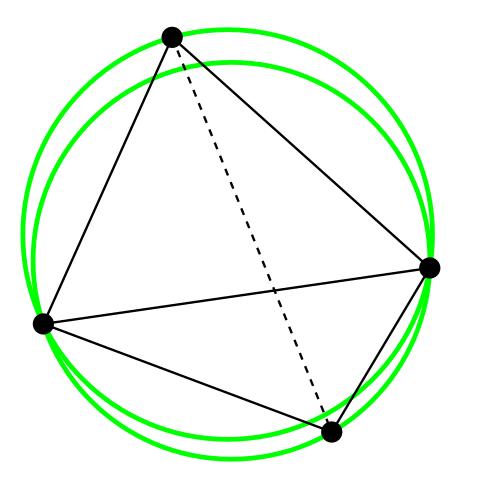
\includegraphics[width=\subfigwidth]{figures/appendix/Edge_Flip_-_Delaunay_condition_ok.png}
        \caption{Flipping the common edge produces a valid Delaunay triangulation for the four points.}\label{subfig:delauneyfix}
    \end{subfigure}
    \caption{Visual Delaunay definition and Flipping.}\label{fig:delauneyflip}
\end{figure}
%
This is an important property because it allows the use of a flipping technique. If two triangles do not meet the Delaunay condition, switching the common edge BD for the common edge AC produces two triangles that do meet the Delaunay condition (see figures~\ref{subfig:delauneyflip}, \ref{subfig:delauneyfix}).
%
This leads to a straightforward algorithm: construct any triangulation of the points, and then flip edges until no triangle is non-Delaunay.